%% LyX 2.0.4 created this file.  For more info, see http://www.lyx.org/.
%% Do not edit unless you really know what you are doing.
\documentclass[oneside,dutch]{amsart}
\usepackage[T1]{fontenc}
\usepackage[latin9]{inputenc}
\usepackage[a4paper]{geometry}
\geometry{verbose,tmargin=3cm,bmargin=3cm,lmargin=2cm,rmargin=2cm}
\setlength{\parskip}{\smallskipamount}
\setlength{\parindent}{0pt}
\usepackage{amsthm}
\usepackage{amssymb}
\usepackage{graphicx}
\graphicspath{{Figures/}}

\makeatletter
%%%%%%%%%%%%%%%%%%%%%%%%%%%%%% Textclass specific LaTeX commands.
\numberwithin{equation}{section}
\numberwithin{figure}{section}

\makeatother

\usepackage{babel}
\begin{document}

\title{Een Shimizu nevelkamer voor HiSparc}


\author{N.G. Schultheiss}

\maketitle

\section{Inleiding}

In 1921 bouwde Takeo Shimizu een nevelkamer door een zuiger met een
frequentie rond de 3Hz in een cilinder te laten trillen. Bij iedere
expansie waren er nevelsporen te zien, tenminste als er deeltjes waren.
Met een dergelijke opstelling is het mogelijk om af en toe een deeltje
waar te nemen als er een co�ncidentie in de HiSparc-detectoren plaats
vindt. Door de expansie niet met een zuiger te laten plaatsvinden
maar met een (sauna)luidspreker, is deze aan de co�ncidentie te koppelen.


\section{Specificaties en verwachtingen}

De expansiefactor die met de luidspreker moet worden bereikt licht
in de orde van 1,3. De onderdruk die moet worden bereikt is bijgevolg
ongeveer 250hPa. Uitgaande van een diameter van 10cm, wordt de kracht
op de luidspreker $\triangle p*\frac{1}{4}\pi d^{2}=250*10^{2}*\frac{1}{4}\pi(0,10)^{2}\thickapprox200\mathrm{N}$.

Een eerste onderzoeksvraag is dus of een luidspreker een kracht van
200N kan leveren.

De atmosfeer in de nevelkamer is verzadigd. Het wordt dus een natte
boel. De opstelling moet hier tegen kunnen. Vandaar dat ik een sauna
luidspreker wil gebruiken. Deze kan de vochtigheid hoogst waarschijnlijk
aan. 

\begin{figure}[h]
\noindent \begin{centering}
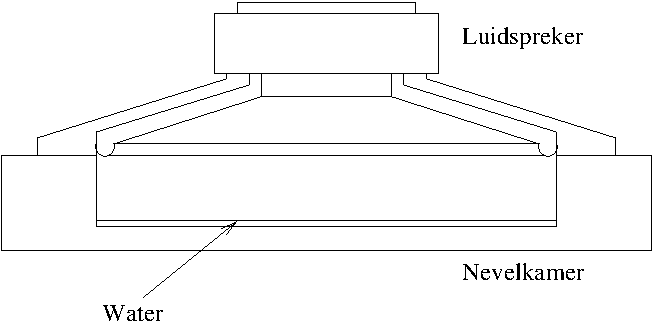
\includegraphics[scale=0.75]{opstelling}
\par\end{centering}

\caption{De opstelling}
\end{figure}


Het is de vraag of de opstelling op deze manier werkt. De muonen hebben
waarschijnlijk enige moeite om door de magneet te komen. Om dit te
voorkomen kan de opstelling op zijn kop worden gezet. Helaas kan er
dan een waterlaag op de luidspreker komen. Een tweede onderzoeksvraag
is of de opstelling werkt en of deze om te keren is.

Met twee webcams met de kijkrichtingen loodrecht op elkaar kan de
richting van de deeltjes worden bepaald. Naast een tijdsverschil bij
de co�ncidenties is er nu een tweede methode om de richting van een
shower te bepalen.

Als de deeltjesdichtheid in de shower homogeen is, is de kans dat
er bij een co�ncidentie een deeltje in de nevelkamer wordt waargenomen
$\frac{oppervlak_{nevelkamer}}{oppervlak_{detectorplaat}}=1.5\%$.
Globaal vindt er in de nevelkamer 1 op de 60 co�ncidenties een waarneming
plaats. 


\section{Aansturing en verwerking}

De luidspreker kan met een versterker worden aangestuurd. De versterker
versterkt een puls die door de co�ncidentie wordt gegenereerd. Daarnaast
moeten de gegevens verwerkt worden, hiervoor is een computer nodig.
De computer verwerkt de beelden uit de beide webcams.
\end{document}
